\documentclass[border=2pt]{standalone}
\usepackage[T1]{fontenc}\usepackage{mathptmx}
\usepackage{amsmath,amssymb}\usepackage{tikz}\usepackage{pgfplots}
\pgfplotsset{compat=1.18}
\usetikzlibrary{shapes.geometric, arrows.meta, positioning, calc}
\setlength{\columnwidth}{3.45in}
\newcommand{\Pfree}{P_{\mathrm{free}}}\newcommand{\dfree}{d_{\mathrm{free}}}\newcommand{\pos}{\mathrm{pos}}
\newcommand{\ind}{\mathbf{1}}\newcommand{\Lin}{\mathcal{L}}
\pgfplotsset{ieeeplot/.style={width=\columnwidth, height=5.4cm,
 tick label style={font=\footnotesize}, label style={font=\footnotesize},
 legend style={font=\footnotesize, draw=black!60, fill=white, fill opacity=0.9, text opacity=1},
 grid=both, grid style={line width=0.2pt, draw=black!15}, major grid style={line width=0.3pt, draw=black!25},
 every axis plot/.append style={line width=0.8pt, mark size=2.2pt}}}
\begin{document}
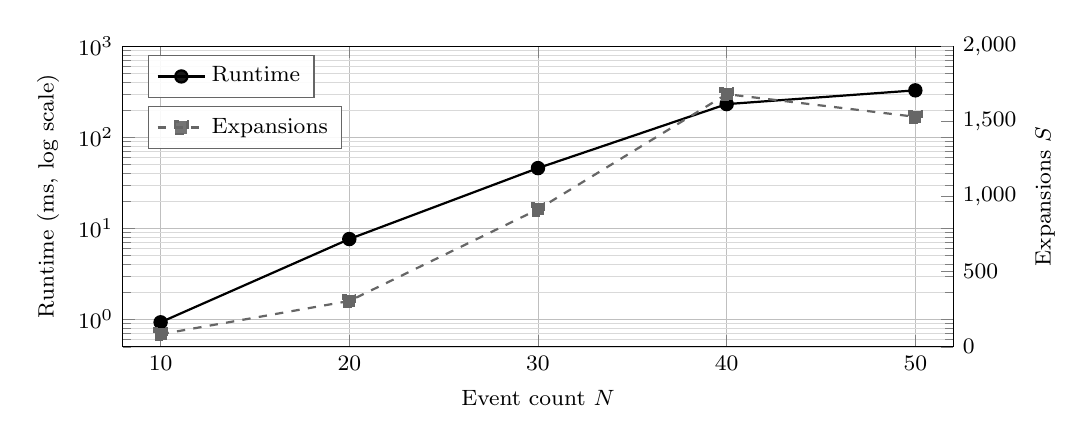
\begin{tikzpicture}
\begin{axis}[ieeeplot, name=rt,
  xlabel={Event count $N$}, ylabel={Runtime (ms, log scale)},
  xmin=8, xmax=52, xtick={10,20,30,40,50},
  ymode=log, ymin=0.5, ymax=1000,
  legend style={at={(0.03,0.97)}, anchor=north west}, legend cell align=left]
\addplot[black, solid, mark=*] coordinates {(10,0.93) (20,7.63) (30,45.84) (40,231.12) (50,327.37)};
\addlegendentry{Runtime}
\end{axis}
\begin{axis}[ieeeplot, at={(rt.south west)}, anchor=south west,
  axis y line*=right, axis x line=none, ylabel={Expansions $S$},
  xmin=8, xmax=52, ymin=0, ymax=2000, grid=none,
  legend style={at={(0.03,0.80)}, anchor=north west}, legend cell align=left]
\addplot[black!60, dashed, mark=square*] coordinates {(10,83.7) (20,305.0) (30,914.5) (40,1681.0) (50,1530.3)};
\addlegendentry{Expansions}
\end{axis}
\end{tikzpicture}
\end{document}
